\section{Durchführung}
\label{sec:Durchführung}
Der Aufbau wird in \autoref{fig:Abb_2} dargestellt, wobei der He-Ne-Laser im Aufbau nicht um die Strahlachse schwenkbar ist.
\begin{figure}[H]
    \centering
    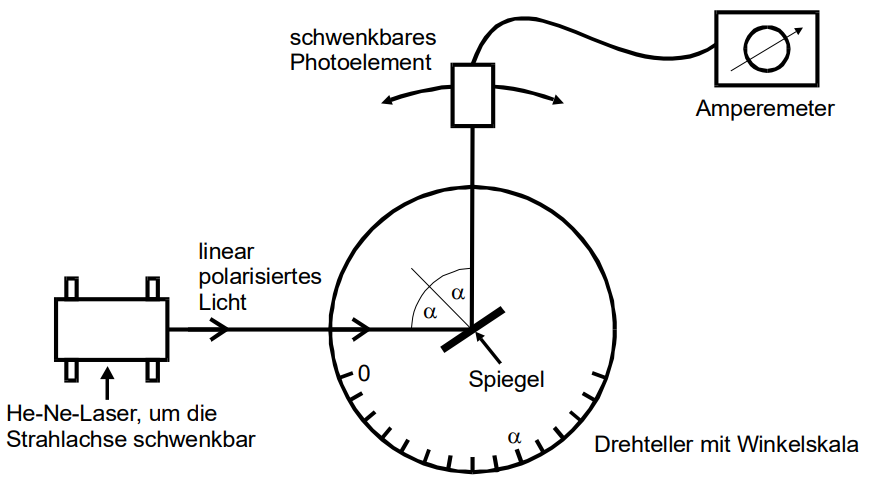
\includegraphics[width=0.5\textwidth]{Abbildung/Abb_2.png}
    \caption {Schematische Darstellung der verwendeten Messapparatur \cite{V407}.}
    \label{fig:Abb_2}
\end{figure}
Vor der eigentlichen Messung muss die Messapparatur richtig justiert werden. Dazu wird der 
Silizium-Spiegel entfernt und eine Messung der Intensität des Laser-Strahls durchgeführt.
Anschließend wird der Spiegel auf den Probenhalter montiert und so kallibriert, dass der Laserstrahl
direkt auf den Laserkopf zurück reflektiert wird. Das Goniometer soll in dieser 
Stellung auf $\qty{0}{\degree}$ zeigen. Der Spiegel wird auf dem Drehteller fixiert und die Messung kann beginnen.\\
Für die eigentliche Messung wird der Winkel für die Polarisation am Polarisationsfilter, der sich im Lichtweg des Lasers befindet eingestellt.
Es Messungen bei Polarisationswinkeln von $\qty{0}{\degree}$ und $\qty{90}{\degree}$  durchgeführt.
Die Intensität des reflektierten Laserstrahls wird für unterschiedliche Eintrittswinkel gemessen und 
in eine Tabelle eingetragen. Das Winkelintervall geht hierbei von $\qty{4}{\degree}$ bis $\qty{87}{\degree}$.
Dabei werden die Messwerte in einem Abstand von $\qty{2}{\degree}$ aufgenommen.